% Overleaf: upload this file, set it as the Main document, and use pdfLaTeX.
% Self-contained: no dataset, image file, .bib file, or shell escape is required.
% The bibliography is embedded below. Compile twice for references and contents.
\documentclass[11pt,letterpaper]{article}

\usepackage[T1]{fontenc}
\usepackage[utf8]{inputenc}
\usepackage{lmodern}
\usepackage[margin=1in]{geometry}
\usepackage{microtype}
\usepackage{amsmath,amssymb}
\usepackage{booktabs,longtable,tabularx,array}
\usepackage{enumitem}
\usepackage{needspace}
\usepackage{xcolor}
\usepackage{tikz}
\usetikzlibrary{arrows.meta,positioning}
\usepackage{xurl}
\usepackage{fancyhdr}
\usepackage{listings}
\definecolor{navy}{HTML}{17365D}
\definecolor{teal}{HTML}{216869}
\definecolor{lightblue}{HTML}{F0F5F8}
\usepackage[colorlinks=true,linkcolor=navy,citecolor=teal,urlcolor=teal,
  pdftitle={Oceanographic Profiles from GO-SHIP P02W (2022)},
  pdfauthor={LEC2026 Faculty AI Workshop}]{hyperref}

\newcolumntype{L}[1]{>{\raggedright\arraybackslash}p{#1}}
\newcolumntype{Y}{>{\raggedright\arraybackslash}X}
\newcommand{\field}[1]{\nolinkurl{#1}}
\newcommand{\degC}{\ensuremath{{}^{\circ}\mathrm{C}}}
\newcommand{\SP}{\ensuremath{S_{\mathrm{P}}}}
\newcommand{\dbar}{\ensuremath{\mathrm{dbar}}}
\setlength{\parskip}{5pt}
\setlength{\parindent}{0pt}
\setlength{\headheight}{14pt}
\setlength{\emergencystretch}{2em}
\setlist[itemize]{topsep=3pt,itemsep=2pt}
\setlist[enumerate]{topsep=3pt,itemsep=3pt}
\renewcommand{\arraystretch}{1.17}
\pagestyle{fancy}
\fancyhf{}
\fancyhead[L]{\small GO-SHIP P02W: dataset and analysis plan}
\fancyhead[R]{\small LEC2026}
\fancyfoot[C]{\thepage}
\lstset{basicstyle=\ttfamily\footnotesize,breaklines=true,
  columns=fullflexible,keepspaces=true,showstringspaces=false,
  frame=single,rulecolor=\color{lightblue},backgroundcolor=\color{lightblue},
  xleftmargin=3pt,xrightmargin=3pt,aboveskip=8pt,belowskip=8pt}

\title{\textbf{Oceanographic Profiles from\newline GO-SHIP P02W (2022)}\\[6pt]
  \large Dataset Description, Data Dictionary,\newline and Educational Analysis Plan}
\author{LEC2026 Faculty AI Workshop}
\date{October 23, 2026}

\begin{document}
\maketitle
\thispagestyle{empty}

\begin{abstract}
This report documents a small, reproducible oceanographic dataset selected for a faculty workshop on AI-assisted scientific analysis. The teaching file contains 682 pressure-level records from three conductivity--temperature--depth (CTD) casts collected during the 2022 GO-SHIP P02W cruise aboard R/V \emph{Roger Revelle}. Twelve fields retain cruise and profile identity, sampling time and location, sea-water pressure, in-situ temperature, Practical Salinity, and the source's temperature and salinity quality flags. A conservative workshop policy retains 679 records and excludes three interpolated surface values.

The analytical goal is to describe vertical temperature and salinity structure, compare two common pressure bands, and build an interactive profile-viewing tool whose choices remain visible and reproducible. The educational goal is to help faculty specify a scientific task, use AI to implement a targeted modification, and evaluate the resulting code and interpretation. The dataset is a selected collection of profiles at different locations and dates. It supports descriptive comparisons of those profiles; it does not by itself establish a warming trend, a causal mechanism, or a regional climatology. The report provides the complete input data dictionary, quality-control definitions, reference summaries, analysis formulas, tool specifications, and interpretation limits.
\end{abstract}

\begin{center}
\small
\begin{tabular}{ll}
\toprule
\textbf{Cruise identifier} & \field{33RR20220430} \\
\textbf{Teaching subset} & Stations 3, 50, and 100; cast 1; pressure $\leq 600$ dbar \\
\textbf{File} & \field{p02w_upper600_erddap.csv} \\
\textbf{Snapshot retrieved} & October 13, 2026 \\
\textbf{Report and source review} & October 23, 2026 \\
\textbf{Companion notebook} & \field{02_oceanography.ipynb} \\
\bottomrule
\end{tabular}
\end{center}

\clearpage
\tableofcontents
\clearpage

\section{Purpose and scope}
\label{sec:purpose}

The workshop uses an authentic scientific problem: how can a researcher turn a small collection of ocean profiles into an analysis that another person can inspect, reproduce, and question? Participants begin with measured or scientifically processed quantities and documented metadata. They then examine the relationship between an analysis question, its implementation, and the claim made from its output.

The central question is:
\begin{quote}
How do in-situ temperature and Practical Salinity vary with sea-water pressure in three selected casts, and how do the observed comparisons depend on quality-control and sampling-coverage choices?
\end{quote}

The intended product is a transparent analysis tool rather than a predictive model. Its inputs are the selected station, displayed variable, pressure limit, interpolation policy, and optional display smoothing. Its outputs are labelled profiles, descriptive summaries, and a record of the choices used to produce them. An AI assistant can help write or modify the implementation, while the faculty member supplies scientific definitions, checks the transformation, and decides what the result supports.

This report distinguishes three levels of evidence throughout:
\begin{enumerate}
  \item \textbf{Source documentation:} the cruise identity, variable definitions, measurement scales, and quality conventions declared by the data providers.
  \item \textbf{Snapshot facts:} counts, coordinates, observed ranges, and summaries calculated from the local teaching CSV.
  \item \textbf{Workshop choices:} the station selection, acceptance rule, comparison bands, plotting controls, and proposed learning activities.
\end{enumerate}
The third category should not be mistaken for a rule imposed by the original investigators. In particular, retaining only quality flag 2 is a deliberately simple teaching policy, not a general assertion that every other flag denotes unusable data.

\section{Scientific background and collection context}

\subsection{GO-SHIP and the P02W cruise}
GO-SHIP, the Global Ocean Ship-based Hydrographic Investigations Program, coordinates repeated ship-based sections used to study ocean properties and their changes. The broader program collects physical and biogeochemical observations across ocean basins and through the water column. A repeated observing program can support change-detection studies when observations are appropriately matched and evaluated; the three-profile selection used here is only a small educational excerpt from that setting.\cite{goship}

CCHDO identifies cruise \field{33RR20220430} as the 2022 P02W occupation, within the P02 section, aboard R/V \emph{Roger Revelle}. The cruise ran from April 30 to June 10, 2022. Alison Macdonald was chief scientist and Shuwen Tan was co-chief scientist.\cite{cruise} The selected casts span May 4 to June 3. Their differing times are relevant metadata, but do not turn the dataset into a time series at a fixed location.

\subsection{What a CTD measures}
CTD is the conventional abbreviation for conductivity--temperature--depth. In this application, the vertical coordinate carried into the analysis is \emph{pressure}, measured in decibars, rather than an independently measured depth in metres. Temperature is reported on the International Temperature Scale of 1990 (ITS-90). Practical Salinity is a derived conductivity-related quantity reported on the Practical Salinity Scale of 1978 (PSS-78).

The cruise report describes an SBE9+ CTD system, pressure measurement, paired temperature and conductivity sensors, and a 36-bottle rosette. It also describes processing into a two-decibar downcast pressure series.\cite{cruisereport} The workshop CSV therefore represents a processed scientific product. Its rows should not be described as original high-frequency instrument scans. Nor should the table be confused with bottle samples, Argo float measurements, satellite sea-surface temperatures, or an interpolated global climatology.

In general, CTD processing involves sensor response considerations, calibration, quality assessment, and averaging or other reduction to a pressure series.\cite{ctdmanual} Those upstream procedures are not repeated in the teaching notebook. The notebook starts from the archived values and flags; it performs a separate, explicitly stated acceptance and display workflow.

\subsection{Quantities deliberately outside the exercise}
The selected file does not include conductivity itself, dissolved oxygen, nutrients, bottle sample measurements, current velocities, density, or uncertainty estimates for individual measurements. It also does not include potential temperature, Conservative Temperature, or Absolute Salinity. Those quantities require additional definitions, inputs, or calculations and should not be inferred merely by renaming columns.

For example, \SP\ is dimensionless and is not Absolute Salinity expressed in grams per kilogram.\cite{gswsalinity} Similarly, an in-situ temperature profile is not automatically a potential-temperature profile. Maintaining the exact meaning of a quantity is one of the main scientific responsibilities in AI-assisted code editing.

\section{Data sources, selection, and provenance}

\subsection{The source chain}
The observations were collected by the cruise investigators, archived and documented through CCHDO, and accessed for this workshop through NOAA Pacific Marine Environmental Laboratory's ERDDAP table \field{cchdo_ctd}. The cruise archive supplies cruise-specific context and data history; ERDDAP supplies convenient variable selection, row constraints, and machine-readable metadata.\cite{cruise,erddap}

\begin{figure}[htbp]
\centering
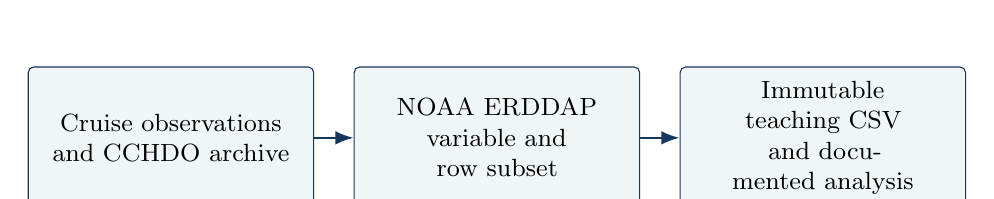
\begin{tikzpicture}[
  box/.style={draw=navy,rounded corners=2pt,fill=lightblue,
    text width=0.27\linewidth,minimum height=18mm,align=center,
    inner sep=5pt,font=\small},
  >=Latex,node distance=5mm]
  \node[box] (a) {Cruise observations\\and CCHDO archive};
  \node[box,right=of a] (b) {NOAA ERDDAP\\variable and row subset};
  \node[box,right=of b] (c) {Immutable teaching CSV\\and documented analysis};
  \draw[->,thick,navy] (a) -- (b);
  \draw[->,thick,navy] (b) -- (c);
\end{tikzpicture}
\caption{Provenance chain for the educational dataset. The local snapshot preserves the retrieved CSV; the notebook applies its acceptance policy to a separate in-memory table.}
\label{fig:lineage}
\end{figure}

\subsection{Exact selection}
The download projects the source table to the twelve columns listed in Section~\ref{sec:dictionary} and applies these constraints:
\begin{itemize}
  \item cruise \field{expocode} equals \field{33RR20220430};
  \item \field{station} matches 3, 50, or 100;
  \item \field{cast} equals 1;
  \item \field{pressure} is no greater than 600 dbar.
\end{itemize}
The original selection does not impose a nonnegative pressure constraint in the request itself. The local acceptance rule subsequently requires pressure between 0 and 600 dbar. All records in the supplied snapshot already satisfy that range.

The stations were selected for a manageable, contrasting classroom example. They are not a random sample of the Pacific Ocean or a statistically representative subsample of the entire cruise. There is one selected cast per station. The actual selected values, time coverage, and row counts are established from the CSV, not from the aggregate ERDDAP collection's global range attributes.

\subsection{Snapshot identity and file structure}
\label{sec:snapshot}
The source file was retrieved on October 13, 2026. Its size is 83,028 bytes, approximately 81 KiB. The checksum recorded in the workshop provenance file is:
\begin{quote}
\small\url{8edc63a57d031cff681540033ff3efb29fca727f01504db880adb6f8f49450ea}
\end{quote}
This is a SHA-256 checksum of the original CSV bytes. It identifies the teaching snapshot; it is not a measure of the scientific accuracy of its observations. The file contains one header record, one units record, and 682 observation records.

The file is retained as retrieved, including the units row. In the workshop folder it is located at:
\begin{quote}
\small\field{workshop/data/oceanography/p02w_upper600_erddap.csv}
\end{quote}
The corresponding \field{provenance.json} retains the request URL, access date, credit, selected variables, and checksum. Dataset files are managed separately from the GitHub teaching source. A reader can use the documented request to obtain data locally without embedding the observations in this report.

\subsection{Archive revisions and reproducibility}
Source archives can be corrected after collection. CCHDO's cruise history records later CTD reprocessing, including an August 19, 2026 update.\cite{cruise} The original cruise report predates such updates. Consequently, its initial processing account should not be treated as the complete version history of every value in a later download.

The practical reproducibility target is the October 13 snapshot and its hash. A new download should be compared with that identity before reproducing the reference summaries in Section~\ref{sec:reference}. A changed hash calls for inspection and documentation; it does not by itself establish an error in either file. The provider pages were reviewed for this report on October 23, 2026.

\subsection{Access, rights, and credit}
The NOAA ERDDAP endpoint declares CC0-1.0 for the distributed dataset.\cite{erddap} The workshop retains scientific attribution to CCHDO, GO-SHIP P02W, NOAA PMEL ERDDAP, the cruise investigators, and the vessel. CCHDO explains that its aggregate holdings are openly available and that citation of the applicable archive snapshot and individual cruises remains an expected scientific practice.\cite{license,citation}

The references in this report provide traceable source links. For a journal submission, obtain the applicable archive snapshot DOI and any cruise-specific requested citation from CCHDO's current citation guidance.

\section{Observational unit and sampling geometry}
\label{sec:unit}

\subsection{One row, one profile, and one station}
A row represents a pressure level within a processed cast. Its temperature and salinity describe the archived values at that pressure coordinate. The pressure levels are nested within profiles; the profiles are associated with selected stations on one cruise.

\begin{center}
\begin{tabularx}{\linewidth}{L{0.22\linewidth}Y}
\toprule
\textbf{Level} & \textbf{Meaning in this file} \\
\midrule
Cruise & One expedition identifier: \field{33RR20220430}. \\
Station & One of three selected station identifiers: 3, 50, or 100. \\
Cast/profile & One selected deployment, cast 1, at each station. \\
Pressure-level row & One processed level in that cast's vertical series. \\
\bottomrule
\end{tabularx}
\end{center}

The natural row key for this snapshot is the pair
\field{(profile_id, pressure)}. No duplicate pairs or exact duplicate observation records are present. There are 682 source rows but only three selected profiles. These counts answer different questions and must not be substituted for one another when discussing replication.

\subsection{Location, time, and record counts}
Table~\ref{tab:stations} gives the actual profile metadata. Coordinates and UTC times are constant across rows within each selected profile. The timestamp is therefore used as profile metadata, not as an independently varying timestamp for every pressure-level observation.

\begin{table}[htbp]
\centering\small
\caption{Selected profile locations, times, and record counts from the teaching snapshot. Longitude uses the signed degrees-east representation in the CSV.}
\label{tab:stations}
\begin{tabular}{rllrr}
\toprule
\textbf{Station} & \textbf{UTC date and time} & \textbf{Latitude, longitude} & \textbf{Raw} & \textbf{Accepted} \\
\midrule
3 & 2022-05-04 18:58 & $32.5070,\ 133.0290$ & 80 & 79 \\
50 & 2022-05-19 02:33 & $30.0006,\ 161.0654$ & 301 & 300 \\
100 & 2022-06-03 05:05 & $30.0002,\ -171.0212$ & 301 & 300 \\
\midrule
Total & & & 682 & 679 \\
\bottomrule
\end{tabular}
\end{table}

Station 100's longitude is $171.0212^{\circ}$ west, equivalently $188.9788^{\circ}$ east on a 0--360-degree convention. This matters when mapping the observations or drawing a track across the date line. Station identifiers are labels, not distances, elapsed times, or equally spaced geographic coordinates.

\subsection{Pressure coverage and the meaning of a truncated profile}
\begin{table}[htbp]
\centering
\caption{Pressure coverage in the source and accepted tables. Pressure spacing between consecutive retained levels is 2 dbar in every selected profile.}
\label{tab:coverage}
\begin{tabular}{rrrr}
\toprule
\textbf{Station} & \textbf{Source range, dbar} & \textbf{Accepted range, dbar} & \textbf{Accepted levels} \\
\midrule
3 & 0--158 & 2--158 & 79 \\
50 & 0--600 & 2--600 & 300 \\
100 & 0--600 & 2--600 & 300 \\
\bottomrule
\end{tabular}
\end{table}

For stations 50 and 100, 600 dbar is the upper bound of the subset request. It is not evidence that the original cast or the ocean ended there. Station 3's selected profile ends at 158 dbar. That fact establishes its coverage in this file; it does not by itself explain why sampling ended, identify bottom depth, or establish the complete sampling history of the station.

No value should be invented to extend station 3 to the requested display limit. When a plot is displayed to 600 dbar, an empty lower region is meaningful evidence of unavailable coverage in the selected series.

\section{Input data dictionary}
\label{sec:dictionary}

The dictionary below covers all twelve columns in their CSV order. CSV entries are textual representations on disk; the recommended analysis types describe how to use them after loading. Source meanings and measurement scales follow the ERDDAP variable attributes.\cite{erddap} Observed values and examples refer only to this workshop snapshot.

\subsection{Identifiers and sampling metadata}
\small
\begin{longtable}{L{0.23\linewidth}L{0.17\linewidth}L{0.51\linewidth}}
\caption{Identifiers, times, and geographic coordinates.}\label{tab:dictionarymetadata}\\
\toprule
\textbf{Column} & \textbf{Type / unit} & \textbf{Definition and analysis guidance} \\
\midrule
\endfirsthead
\multicolumn{3}{l}{\textit{Table \thetable\ continued}}\\
\toprule
\textbf{Column} & \textbf{Type / unit} & \textbf{Definition and analysis guidance} \\
\midrule
\endhead
\bottomrule
\endfoot
\field{expocode} & String; no unit & Cruise identifier, corresponding to WHP \field{EXPOCODE}. Every row is \field{33RR20220430}. Preserve it as text for provenance and joins. Its apparent digits do not make it a numerical explanatory variable. \\
\addlinespace
\field{station} & String; no unit & Station identifier, corresponding to WHP \field{STNNBR}. The observed labels are \field{3}, \field{50}, and \field{100}. The notebook explicitly reads this column as text. Numeric-looking labels should not be averaged or treated as a spatial coordinate. \\
\addlinespace
\field{cast} & Integer identifier; no unit & Cast number at a station, corresponding to WHP \field{CASTNO}. The value is 1 in every selected record. In a larger dataset, station and cruise are needed to interpret it; cast 1 is not globally unique. \\
\addlinespace
\field{profile_id} & String; no unit & Unique profile identifier in the source table. The snapshot contains \field{33RR20220430_3_1}, \field{33RR20220430_50_1}, and \field{33RR20220430_100_1}. Use it to group pressure-level rows; retain the identifier as supplied. \\
\addlinespace
\field{time} & UTC-aware datetime & Profile time coordinate. CSV values use ISO-style timestamps ending in \field{Z}, indicating UTC. There are three distinct values, one per profile. The underlying server time coordinate is expressed as seconds since the Unix epoch, but the CSV already supplies readable timestamps. Do not interpret repeated profile times as sensor sampling times down the cast. \\
\addlinespace
\field{latitude} & Floating point; degrees north & Geographic latitude associated with the profile. Positive values are north of the equator. Snapshot values range from $30.0002$ to $32.5070$. The repeated coordinate is profile metadata; the file does not describe a detailed ship-drift trajectory during a cast. \\
\addlinespace
\field{longitude} & Floating point; degrees east & Geographic longitude associated with the profile. The snapshot includes positive eastern longitudes and a negative value for station 100. Preserve the supplied convention, or explicitly document a conversion when drawing maps across the date line. Longitude is angular, so ordinary subtraction across its wrap can be misleading. \\
\end{longtable}
\normalsize

\Needspace{10\baselineskip}
\subsection{Measurements and associated quality flags}
\small
\begin{longtable}{L{0.23\linewidth}L{0.17\linewidth}L{0.51\linewidth}}
\caption{Pressure, temperature, salinity, and quality-control columns.}\label{tab:dictionarymeasurements}\\
\toprule
\textbf{Column} & \textbf{Type / unit} & \textbf{Definition and analysis guidance} \\
\midrule
\endfirsthead
\multicolumn{3}{l}{\textit{Table \thetable\ continued}}\\
\toprule
\textbf{Column} & \textbf{Type / unit} & \textbf{Definition and analysis guidance} \\
\midrule
\endhead
\bottomrule
\endfoot
\field{pressure} & Floating point; dbar & Sea-water pressure, positive downward; WHP \field{CTDPRS}. The source snapshot ranges from 0 to 600 dbar. It is the vertical coordinate of the processed series, not depth in metres. For plots, higher pressure is displayed lower on the page. \\
\addlinespace
\field{ctd_temperature} & Floating point; \degC, ITS-90 & In-situ sea-water temperature; WHP \field{CTDTMP}. It describes temperature at the reported pressure. It is not potential temperature or Conservative Temperature. Snapshot accepted values range from approximately 6.583 to 23.043\,\degC. Retain its paired quality flag when selecting data. \\
\addlinespace
\field{ctd_temperature_qc} & Integer code; categorical & Source status flag associated with temperature, using the WOCE CTD instrument convention. Only codes 2 and 6 occur here. The default notebook policy accepts 2. The codes are categories, not temperatures, uncertainty estimates, rankings to average, or confidence probabilities. \\
\addlinespace
\field{ctd_salinity} & Floating point; dimensionless, PSS-78 & Practical Salinity, denoted \SP; WHP \field{CTDSAL}. The CSV units row contains \field{1}, meaning dimensionless. Accepted values span approximately 34.024--35.140. Do not label these values g/kg or substitute them directly for Absolute Salinity. Retain the paired salinity flag. \\
\addlinespace
\field{ctd_salinity_qc} & Integer code; categorical & Source WOCE CTD status flag associated with Practical Salinity. The default analysis requires this flag and the temperature flag to equal 2 on the same row. Agreement of the two flags is observed in this snapshot but must not be assumed for another dataset. \\
\end{longtable}
\normalsize

\subsection{Units, missing values, and numerical precision}
The second CSV record contains units rather than observations. For example, \field{time} is marked \field{UTC}, pressure is marked \field{dbar}, and Practical Salinity is marked \field{1}. This row must be skipped when parsing the numerical observations. Otherwise, a units string can cause a measurement column to be treated as text.

There are no blank fields in the twelve selected columns of this snapshot, and pressure, temperature, and salinity contain no nonfinite values. The broader source metadata declares missing-value conventions such as NaN for measurement variables and 9 as a fill value for the temperature and salinity quality flags. These declarations matter for future downloads even though they do not generate additional exclusions in this file. Missing or unavailable values must not be converted to zero.

Many stored values contain more decimal digits than are useful for a classroom display. This report rounds temperature and salinity summaries to three decimals. That is a presentation choice, not a claim of measurement accuracy at the third decimal. The selected file has no per-observation standard errors, calibration residuals, or instrument-uncertainty columns.

\subsection{Pressure, depth, and salinity distinctions}
A decibar is a pressure unit: $1\ \mathrm{dbar}=10^{4}\ \mathrm{Pa}$. A depth in metres is a geometric distance. They may be numerically similar over some ranges but are not interchangeable. A pressure-to-height/depth conversion requires an explicit physical convention and latitude; the TEOS-10 Gibbs SeaWater toolbox provides a documented calculation.\cite{gswdepth} No such conversion is performed in this exercise.

Practical Salinity is a conductivity-based quantity whose definition is distinct from a mass fraction.\cite{gswsalinity} The appropriate axis label is ``Practical salinity (PSS-78; dimensionless).'' If an extension computes density or another thermodynamic property, its inputs, pressure reference, salinity conversion, and temperature definition must be documented separately.

\section{Quality control and acceptance policy}
\label{sec:qc}

\subsection{The applicable flag convention}
The source explicitly identifies the quality variables as WOCE CTD instrument flags. Table~\ref{tab:flags} follows the meanings declared in the endpoint and the CCHDO CTD quality-code table.\cite{erddap,qcguide} It is essential to select the convention for the kind of observation being analysed. In CCHDO water-sample tables, for example, code 6 has a replicate-mean interpretation; that is not its interpretation for these CTD columns.

\begin{table}[htbp]
\centering\small
\caption{Declared CTD quality codes and the workshop's default handling. Only 2 and 6 are observed in the selected CSV.}
\label{tab:flags}
\begin{tabularx}{\linewidth}{rYL{0.23\linewidth}}
\toprule
\textbf{Code} & \textbf{Meaning} & \textbf{Default policy} \\
\midrule
0 & No flag assigned & Exclude; inspect source \\
1 & Not calibrated & Exclude \\
2 & Acceptable measurement & Retain if other checks pass \\
3 & Questionable measurement & Exclude \\
4 & Bad measurement & Exclude \\
5 & Not reported & Exclude \\
6 & Interpolated over a pressure interval larger than 2 dbar & Exclude; optional display sensitivity \\
7 & Despiked & Exclude under this simple policy \\
8 & Not used for CTD data & Investigate if encountered \\
9 & Not sampled; also declared as a flag fill value & Exclude \\
\bottomrule
\end{tabularx}
\end{table}

The CCHDO CTD table identifies code 8 as not used for CTD data. It is absent from the temperature/salinity \field{flag_values} mapping displayed by the endpoint and from this snapshot; an occurrence in another file should be investigated rather than accepted. A flag alone does not specify the exact interpolation procedure or the numerical uncertainty of a value. A useful quality-control policy states what it accepts and why, rather than treating flags as an ordered numerical score.

\subsection{Formal definition of the accepted table}
Let $p_i$, $T_i$, and $S_i$ denote pressure, temperature, and Practical Salinity in row $i$, and let $q_{T,i}$ and $q_{S,i}$ be their temperature and salinity flags. A row is retained when all of the following conditions hold:
\begin{align}
q_{T,i}=2,\qquad &q_{S,i}=2, \label{eq:flags}\\
0\leq p_i\leq600,\qquad &-3\leq T_i\leq40,\qquad 0\leq S_i\leq45, \label{eq:ranges}\\
&p_i,\ T_i,\ S_i\ \text{are finite}. \label{eq:finite}
\end{align}
The ranges use dbar, \degC, and dimensionless Practical Salinity respectively, and all boundaries are inclusive. They are broad workshop sanity checks, not calibrated instrument specifications or exhaustive oceanographic validation criteria. Passing them supplements the provider's flags; it does not replace the provider's quality assessment.

Both source flags are enforced even when a user selects only one variable for display. This keeps the core comparison table and default plot policy consistent. It is a deliberate paired-measurement policy; a different project might use variable-specific acceptance rules, but should state that change explicitly.

\subsection{What is removed in the teaching snapshot}
The source contains 679 rows with flag pair $(2,2)$ and three rows with flag pair $(6,6)$. All three excluded rows are at 0 dbar, one per selected profile. No additional row fails the finite-value or broad-range checks. Therefore,
\[
682\ \text{source records} - 3\ \text{flag exclusions}
=679\ \text{accepted records}.
\]
Approximately 99.56\% of the source rows are retained. Each excluded 0-dbar record has the same stored temperature and salinity pair as the 2-dbar record in that profile. This observation is consistent with a reason to inspect the source flags carefully; it does not justify assigning an undocumented interpolation algorithm.

The excluded values are not labelled as independent, acceptable surface measurements. They remain in the unchanged source file and can be included in a clearly labelled display sensitivity check. Because the formal comparison bands begin at 2 dbar, adding these 0-dbar rows does not change the reference band means defined below.

\section{The scientific and educational goals}
\label{sec:goals}

\subsection{Scientific goal: a bounded descriptive comparison}
The exercise aims to characterize these selected profiles rather than estimate a population parameter for the Pacific. The primary questions are:
\begin{enumerate}
  \item How does in-situ temperature vary with pressure within each cast?
  \item How does Practical Salinity vary over the same sampled range?
  \item Within each cast, how do mean temperatures in 2--50 dbar and 100--150 dbar differ?
  \item Which differences remain visible when all casts are compared over a common pressure interval?
  \item How do inclusion of interpolated values, smoothing, and incomplete coverage change the presentation or a proposed interpretation?
\end{enumerate}
These questions are answerable with transparent filtering, plotting, and arithmetic summaries. They do not require a trained machine-learning model or a language model to perform the numerical calculations.

\subsection{Educational goal: make analytical choices explicit}
For faculty with little coding experience, the problem provides a concrete setting in which to practice six skills:
\begin{enumerate}
  \item \textbf{Translate a question into a data requirement:} identify the variable, profile, coordinate, and valid comparison range.
  \item \textbf{Read metadata before analysing:} recognize units, measurement scales, flag conventions, and the nested observational unit.
  \item \textbf{Separate data quality from appearance:} understand why a smooth line can conceal unsupported values or absent coverage.
  \item \textbf{Use a reusable tool:} change explicit function inputs rather than manually editing observations.
  \item \textbf{Direct an AI assistant precisely:} request one modification while preserving the scientific assumptions and output requirements.
  \item \textbf{Evaluate the resulting claim:} distinguish a description of selected casts from an unsupported temporal, causal, or regional conclusion.
\end{enumerate}

\subsection{Success criteria}
The exercise is successful when a participant can explain what one row represents, identify which records were excluded, state the units on a plot, describe station 3's shorter observed coverage and its consequences for comparison, and justify the chosen comparison bands. A satisfactory tool must show its station and date, preserve the flags and source values, expose absent coverage, and produce results consistent with its stated settings.

The result of interest is not simply that an AI-generated cell runs. The participant should also be able to identify a plausible-looking interpretation that the data do not support and explain what additional evidence would be needed.

\section{Proposed analysis workflow}
\label{sec:methods}

\subsection{Load and inspect before plotting}
The notebook first locates the local CSV, with a documented source-download fallback if the file is absent. It reports the checksum and parses the observations after skipping the units row. It retains station and profile identifiers as text, and parses \field{time} as a UTC-aware datetime.

Initial inspection should confirm the twelve expected columns, one selected cruise, three distinct profiles, expected station/cast combinations, and the distribution of quality-flag pairs. Additional structural checks include nonfinite measurements, duplicate profile--pressure keys, metadata consistency within profiles, and the pressure spacing after the acceptance policy is applied.

\subsection{Plot profiles on their measured coordinate}
The first figure places temperature and Practical Salinity in separate panels with a shared pressure coordinate. Each line joins pressure levels from one cast; it does not connect observations across stations into a time series. Pressure increases downward on the page, and the legend shows station and date. Axis labels retain ITS-90 and PSS-78 conventions.

Start with the accepted unsmoothed values. A profile can contain small reversals or fine structure, so neither monotonic temperature nor monotonic salinity should be imposed as a prerequisite for plotting. The figure is a description of available observations, not a diagram of an idealized ocean.

\subsection{Define comparable pressure bands}
Let $s$ denote a selected station and $B=[a,b]$ an inclusive pressure band. Define the accepted index set
\begin{equation}
\mathcal{I}_{s,B}=\{i:\ s_i=s,\ a\leq p_i\leq b,\ i\ \text{satisfies Eqs.~\eqref{eq:flags}--\eqref{eq:finite}}\}.
\end{equation}
With $n_{s,B}=|\mathcal{I}_{s,B}|$, the descriptive temperature mean is
\begin{equation}
\overline{T}_{s,B}=\frac{1}{n_{s,B}}\sum_{i\in\mathcal{I}_{s,B}}T_i,
\qquad n_{s,B}>0.
\label{eq:mean}
\end{equation}
The same arithmetic definition can summarize \SP. These means are averages of accepted pressure-level values in the selected series. They are not ocean-volume averages, area-weighted means, heat-content estimates, or averages of independent station replicates.

The workshop chooses
\[
B_U=[2,50]\ \mathrm{dbar},\qquad B_L=[100,150]\ \mathrm{dbar}.
\]
All three accepted profiles cover both bands. On the observed 2-dbar grid, the upper band contributes $(50-2)/2+1=25$ levels and the lower band contributes $(150-100)/2+1=26$. Inclusive boundaries must be retained to reproduce these counts.

\subsection{Define the temperature contrast and its sign}
The comparison is lower-band mean minus upper-band mean:
\begin{equation}
\Delta T_s=\overline{T}_{s,B_L}-\overline{T}_{s,B_U}.
\label{eq:contrast}
\end{equation}
A negative value means the higher-pressure band is cooler on average in that cast. The units are \degC. The statistic is a contrast between two band means, not a vertical gradient, a cooling rate through time, or a causal effect. The bands are chosen for a reproducible comparison; they are not an algorithmic estimate of mixed-layer depth or thermocline boundaries.

\subsection{Coverage checks and an implementation qualification}
The current \field{band_summary} function checks that a profile's accepted minimum and maximum pressures bracket the requested band. If they do not, it returns zero contributing samples and unavailable means. The output name \field{complete_band_coverage} should be read in that specific implementation sense.

\textbf{Bracketing is not a general interior-gap test.} A profile could satisfy the minimum/maximum condition while lacking pressure levels inside the interval. An independent inspection of this snapshot finds uninterrupted 2-dbar spacing in each accepted series and the expected 25 and 26 observations in the two comparison bands. For another download or another QC policy, count expected levels and inspect internal gaps before claiming complete coverage.

A useful demonstration requests 500--600 dbar. Stations 50 and 100 provide 51 accepted levels each, whereas station 3 cannot support that band. Reporting ``unavailable'' for station 3 preserves the distinction between no observation and a measured zero.

\section{Reference descriptions of the fixed snapshot}
\label{sec:reference}

The following summaries describe the original October 13, 2026 teaching file under the strict policy. They were independently calculated from that CSV for this report and checked against the existing temperature-summary export. They are reference values for review, not evidence of a broader inferential study. The full notebooks were not rerun for this report.

\subsection{Observed ranges}
\begin{table}[htbp]
\centering
\caption{Observed ranges after acceptance. The raw and accepted temperature/salinity extrema happen to be identical in this snapshot. Values are rounded to three decimals.}
\label{tab:ranges}
\begin{tabular}{rrr}
\toprule
\textbf{Station} & \textbf{Temperature range, \degC} & \textbf{Practical Salinity range} \\
\midrule
3 & 15.200--20.687 & 34.477--34.689 \\
50 & 8.776--23.043 & 34.097--34.997 \\
100 & 6.583--22.515 & 34.024--35.140 \\
\bottomrule
\end{tabular}
\end{table}

Ranges over entire available profiles should be interpreted with their unequal pressure coverage in mind. Station 3 ends at 158 dbar, whereas the other selected profiles extend to the 600-dbar query cap. A difference in full-profile extrema therefore combines property differences with differences in the interval sampled.

\subsection{Temperature contrast over common bands}
\begin{table}[htbp]
\centering
\caption{Reference means and the lower-minus-upper temperature contrast. Every station contributes 25 upper-band and 26 lower-band observations.}
\label{tab:temperature}
\begin{tabular}{rrrr}
\toprule
\textbf{Station} & \textbf{2--50 dbar, \degC} & \textbf{100--150 dbar, \degC} & \textbf{$\Delta T$, \degC} \\
\midrule
3 & 19.952 & 15.757 & $-4.195$ \\
50 & 20.387 & 16.714 & $-3.672$ \\
100 & 21.744 & 17.419 & $-4.325$ \\
\bottomrule
\end{tabular}
\end{table}

In each selected cast, the lower band is cooler on average than the upper band. The magnitudes of the three contrasts differ. These are descriptions of the selected casts and chosen bands. They do not identify a mechanism or establish how the ocean changed between the casts' dates.

\subsection{Practical Salinity as complementary context}
\begin{table}[htbp]
\centering
\caption{Additional report summaries of Practical Salinity. These use the same accepted rows and band definitions; the difference is lower minus upper. The notebook's main comparison export reports temperature, while its band-summary helper also returns mean Practical Salinity.}
\label{tab:salinity}
\begin{tabular}{rrrr}
\toprule
\textbf{Station} & \textbf{2--50 dbar, \SP} & \textbf{100--150 dbar, \SP} & \textbf{Difference in \SP} \\
\midrule
3 & 34.496 & 34.605 & $+0.109$ \\
50 & 34.870 & 34.707 & $-0.163$ \\
100 & 35.103 & 34.745 & $-0.357$ \\
\bottomrule
\end{tabular}
\end{table}

The sign of the salinity contrast differs among the selected casts. That is useful descriptive context for a discussion of vertical structure. It is insufficient on its own to assign named water masses, quantify density stratification, or infer an advective mechanism. Those interpretations would require additional methods and evidence.

\section{Specification of the interactive analysis tool}
\label{sec:tool}

The companion notebook implements \field{plot_profile} as a reusable function and exposes its inputs through widgets. A direct function call remains available if the notebook frontend does not render controls. Table~\ref{tab:controls} documents what each control does.

\begin{table}[htbp]
\centering\small
\caption{Inputs and behaviour of the current profile-viewing tool.}
\label{tab:controls}
\begin{tabularx}{\linewidth}{L{0.24\linewidth}L{0.23\linewidth}Y}
\toprule
\textbf{Input} & \textbf{Choices / default} & \textbf{Effect and interpretation} \\
\midrule
\field{station} & 3, 50, 100; default 50 & Selects one profile. It does not interpolate between stations. \\
\field{variable} & Temperature or Practical Salinity; default Temperature & Changes the horizontal quantity and its label. Pressure remains the vertical coordinate. \\
\field{max_pressure} & Widget: 20--600 dbar in steps of 20; default 300 & Limits displayed rows and axis extent. The function itself validates 10--600 dbar. Missing lower coverage is left empty. \\
\field{include_interpolated} & False by default & False accepts both flags equal to 2; True accepts codes 2 or 6 in each flag column. Broad range/finite checks still apply. \\
\field{smooth} & False by default & Adds a centred rolling median of 11 accepted observations as a display aid. Original source values remain visible and unchanged. \\
\bottomrule
\end{tabularx}
\end{table}

An interior 11-observation window spans about 20 dbar on the uninterrupted 2-dbar grid. Edge windows use fewer observations, and a gapped profile would not have the same physical span for a fixed observation-count window. Smoothing is therefore not a change in instrument resolution or an additional set of measurements. It can hide sharp features and should be discussed as a display choice.

The tool's current numerical band comparison uses the strict accepted table. Changing a plotting widget does not silently recompute or redefine the exported default comparison. An extension that exports a selected view should record that view's settings separately from the default analysis metadata.

\section{Role of AI in the exercise}
\label{sec:ai}

\subsection{What the assistant should help produce}
The oceanographic computations are deterministic. AI is used as a coding and explanation assistant, for example to add a second panel, improve a label, build an export button, or explain a function in accessible language. Faculty can evaluate a small requested change against the unchanged original function.

A useful prompt states the input table, scientific definitions, required output, and assumptions that must be preserved. For example:
\begin{quote}
Using the accepted profile table, add a temperature--Practical Salinity plot with a separate colour and date label for each station. Temperature is in-situ ITS-90 degrees Celsius and Practical Salinity is dimensionless PSS-78. Preserve both quality-flag checks. Do not compute density or assign water-mass names. Return one new notebook cell and explain two checks I can make on its output.
\end{quote}

This request confines the modification to a visible, reviewable operation. It also prevents several common semantic substitutions: changing in-situ temperature into a different quantity without calculation, discarding salinity QC when plotting temperature, or presenting an interpretation as though it were directly measured.

\subsection{A demonstration sequence}
\begin{enumerate}
  \item State the scientific question and show the data dictionary before presenting code.
  \item Ask participants to predict how station choice, pressure limit, or interpolation policy will affect the figure.
  \item Run the prepared tool and compare its behaviour with that prediction.
  \item Ask an approved AI assistant for one targeted modification in a new cell.
  \item Inspect the changed code, counts, units, and output alongside the original.
  \item Ask participants to write one supported observation and one claim the data cannot establish.
\end{enumerate}
This sequence makes faculty judgment part of the activity. It avoids treating the model's confident explanation or a polished plot as a substitute for checking the source and implementation.

\subsection{Review criteria for an AI-generated change}
\begin{itemize}
  \item \textbf{Identity:} the intended station, cast, and source file are retained.
  \item \textbf{Selection:} both quality flags and the stated pressure/range policy are preserved, or any requested change is explicit.
  \item \textbf{Semantics:} quantity names, temperature scale, salinity convention, pressure units, and dates remain correct.
  \item \textbf{Coverage:} no absent profile segment is filled or extrapolated without an explicitly justified method.
  \item \textbf{Numerics:} counts and reference means agree with the documented band definitions; zero is distinguished from unavailable.
  \item \textbf{Interpretation:} descriptive comparisons are not rewritten as causal effects, trends, or statistically independent replication.
\end{itemize}

\section{Limits of inference and research extensions}
\label{sec:limitations}

\subsection{Dependence and effective replication}
Neighbouring pressure levels within a cast are related samples of a continuous vertical structure. The 679 retained rows are not 679 independent realizations of the ocean state at separate stations. Treating them as independent station replicates would exaggerate the amount of information available for regional or temporal inference.

No significance test, trend regression, or confidence interval is needed to answer the workshop's descriptive questions. A research analysis requiring uncertainty would need an explicit sampling model, a justified treatment of within-profile dependence, and appropriate measurement and sampling uncertainty information.

\subsection{Location and date change together}
The three casts were collected at different places and dates. A difference between station 3 on May 4 and station 100 on June 3 can reflect spatial structure, temporal variability, sampling choices, or other influences. This design does not identify those contributions separately.

For example, ``the Pacific warmed during the cruise'' is not justified by comparing the selected profiles' temperatures. A more defensible statement is that the chosen upper-band means differ among the sampled casts, with the dates, positions, and band definitions stated. Testing a temporal change would require comparable repeated observations at defined locations or an appropriate repeat-section design, together with seasonal, spatial, and methodological context.

\subsection{Coverage and selection effects}
The 600-dbar cap omits the deeper part of profiles that extend beyond it. Station 3's shorter selected series limits any comparison at greater pressures. The purposive selection of three stations also omits much of the cruise and cannot estimate a regional distribution without a separate sampling design.

Comparing full-profile means would mix differing pressure ranges and therefore answer a different question from comparing matched bands. The common-band approach reduces that particular mismatch, but does not remove spatial or temporal confounding.

\subsection{Physical interpretation requires additional methods}
Temperature and Practical Salinity help describe water-column structure, but the current notebook does not calculate density, heat content, buoyancy frequency, mixed-layer depth, water-mass fractions, or circulation. An extension must introduce the necessary equations and assumptions rather than infer those quantities from labels or a generic AI explanation.

Possible later projects include:
\begin{itemize}
  \item comparing more stations within this cruise while respecting the section geometry;
  \item matching historical repeat occupations with explicit treatment of season and station alignment;
  \item deriving thermodynamic quantities with documented TEOS-10 conversions and pressure references;
  \item evaluating the consequences of different accepted quality categories or interior-gap policies;
  \item adding uncertainty information from the full cruise documentation and calibration records.
\end{itemize}
These are extensions requiring additional decisions, not analyses already completed by the supplied notebook.

\section{Reproducible deliverables and reporting requirements}
\label{sec:deliverables}

The workshop notebook is intended to create four reviewable outputs:
\begin{enumerate}
  \item \field{temperature_salinity_profiles.png}: the original two-panel comparison figure;
  \item \field{accepted_observations.csv}: the 679 rows retained under the strict policy;
  \item \field{temperature_band_comparison.csv}: the station-level temperature band summaries;
  \item \field{analysis_metadata.json}: source URL, source hash, row counts, units, QC policy, comparison bands, and interpretation limits.
\end{enumerate}
For the standard folder layout, these are written under \field{workshop/outputs/oceanography/}. Their generation is separate from retaining the immutable source snapshot. Dataset files, caches, and generated outputs can remain local while the notebook, environment specification, dictionary, and report are version-controlled.

A complete research-facing record would additionally preserve the notebook version or Git commit, package versions, run date, and any deviations from the default parameters. Those items should be recorded when the workflow is executed; the present \field{analysis_metadata.json} export does not by itself contain every one of them. The workshop environment uses Python with NumPy, pandas, matplotlib, and ipywidgets. It does not require a GPU, a paid model endpoint, or Hugging Face inference for the oceanographic calculations.

The reference numbers in this report describe the local CSV and a direct inspection of its contents. They do not certify execution of the complete notebook in CloudBank Classroom or the behaviour of its browser widgets. Classroom execution remains a separate facilitator preparation step.

\appendix
\section{Source query and loading example}
\label{app:query}

The projected variables, in order, are:
\begin{lstlisting}
expocode,station,cast,profile_id,time,latitude,longitude,pressure,
ctd_temperature,ctd_temperature_qc,ctd_salinity,ctd_salinity_qc
\end{lstlisting}
The ERDDAP constraints, before URL encoding, are:
\begin{lstlisting}
&expocode="33RR20220430"
&station=~"3|50|100"
&cast=1
&pressure<=600
\end{lstlisting}
The table endpoint is:
\begin{quote}
\small\url{https://data.pmel.noaa.gov/generic/erddap/tabledap/cchdo_ctd.csv}
\end{quote}
The exact URL-encoded request is retained in the workshop's \field{provenance.json}. A new request is subject to source availability and archive revision; it should not silently replace the fixed snapshot when reproducing a result tied to its checksum.

The following concise loading example illustrates the units-row and identifier handling. It is a documentation example; it does not initiate a download or execute the notebook.
\begin{lstlisting}[language=Python]
from pathlib import Path
import pandas as pd

# Adjust the path for your working directory.
path = Path("workshop/data/oceanography/p02w_upper600_erddap.csv")

# Row 0 is the header; row 1 holds units rather than observations.
raw = pd.read_csv(path, skiprows=[1],
                  dtype={"station": str, "profile_id": str})
raw["time"] = pd.to_datetime(raw["time"], utc=True)

# Next apply the full finite-value, range, and two-flag policy.
# Do not replace missing values with zero.
\end{lstlisting}

\section{Dictionary of key derived outputs}
\label{app:derived}

Derived output fields are calculations or workflow decisions, not additional source measurements. The dictionary below describes the main band-comparison export and related helper outputs.

\small
\begin{longtable}{L{0.28\linewidth}L{0.13\linewidth}L{0.50\linewidth}}
\caption{Derived fields and their interpretation.}\label{tab:derived}\\
\toprule
\textbf{Field} & \textbf{Type / unit} & \textbf{Meaning} \\
\midrule
\endfirsthead
\multicolumn{3}{l}{\textit{Table \thetable\ continued}}\\
\toprule
\textbf{Field} & \textbf{Type / unit} & \textbf{Meaning} \\
\midrule
\endhead
\bottomrule
\endfoot
\field{station} & String & Selected station label; the export's index identifier. \\
\field{complete_band_coverage} & Boolean & In the current comparison export, the lower-band bracketing result from the helper. True means accepted minimum/maximum pressures bracket that band. It is not an internal-gap test and does not independently certify upper-band completeness. Both bands have been checked for this snapshot. \\
\field{lower_band_samples} & Integer count & Number of accepted observations contributing to 100--150 dbar, inclusive; 26 at every selected station. It counts pressure levels, not independent casts. \\
\field{upper_band_samples} & Integer count & Number of accepted observations contributing to 2--50 dbar, inclusive; 25 at every selected station. \\
\field{upper_mean_C} & Floating point; \degC & Arithmetic mean of accepted in-situ temperatures in the upper band. \\
\field{lower_mean_C} & Floating point; \degC & Arithmetic mean of accepted in-situ temperatures in the lower band. \\
\field{lower_minus_upper_C} & Floating point; \degC & \field{lower_mean_C} minus \field{upper_mean_C}; the contrast in Eq.~\eqref{eq:contrast}. \\
\field{mean_temperature_C} & Floating point; \degC & Generic temperature mean returned by \field{band_summary} for the requested band; unavailable if the helper's bracketing condition fails. \\
\field{mean_practical_salinity} & Floating point; dimensionless & Generic mean \SP\ returned by the helper for the requested band, using the same accepted rows. It is not a mass-fraction salinity. \\
\field{samples} & Integer count & Generic contributing level count from the helper. When bracketing fails it returns 0, accompanied by unavailable means. \\
\end{longtable}
\normalsize

\section{Brief glossary}
\begin{description}[style=nextline]
  \item[Cast] A sampling deployment of the profiling instrument package. The selected file retains cast 1 at each of three stations.
  \item[CCHDO] The CLIVAR and Carbon Hydrographic Data Office, which assembles and provides documented hydrographic datasets.
  \item[CTD] Conductivity--temperature--depth; the conventional name of the profiling instrument system. Pressure is the measured vertical coordinate used here.
  \item[ERDDAP] A data-serving system that supports requests for selected variables, rows, and output formats.
  \item[ITS-90] The International Temperature Scale of 1990, the temperature reference scale declared for this column.
  \item[PSS-78] The Practical Salinity Scale of 1978. Its Practical Salinity values are dimensionless.
  \item[Profile] A sequence of observations ordered by vertical coordinate within a cast.
  \item[Quality flag] A provider-supplied categorical description of measurement status or processing. It is not a numerical confidence probability.
  \item[Snapshot] A fixed retrieved version of a source file, identified here by access date and SHA-256 checksum.
  \item[Station] A sampling identifier associated with a location in the cruise dataset. The identifier itself is not a coordinate or a physical interval.
\end{description}

\clearpage
\addcontentsline{toc}{section}{References}
\begin{thebibliography}{10}

\bibitem{cruise}
CCHDO. \emph{Hydrographic Cruise: 33RR20220430 (P02W, 2022)}. Cruise identity, investigators, available data, and processing history.
\url{https://cchdo.ucsd.edu/cruise/33RR20220430}.
Accessed October 23, 2026.

\bibitem{erddap}
NOAA Pacific Marine Environmental Laboratory. \emph{ERDDAP information: CCHDO GO SHIP CTD data, dataset cchdo\_ctd}. Variable definitions, measurement scales, WOCE CTD flag mappings, and endpoint license declaration.
\url{https://data.pmel.noaa.gov/generic/erddap/info/cchdo_ctd/index.html}.
Teaching CSV retrieved October 13, 2026; metadata reviewed October 23, 2026.

\bibitem{goship}
GO-SHIP. \emph{About GO-SHIP}. Program objectives, repeat hydrography context, and data acknowledgement guidance.
\url{https://go-ship.org/About.html}.
Accessed October 23, 2026.

\bibitem{cruisereport}
GO-SHIP P02 2022 Hydrographic Program. \emph{Cruise Report for the 2022 Reoccupation of P02W}. Cruise instrumentation, program descriptions, and initial CTD processing account; documentation available through CCHDO.
\url{https://cchdo.ucsd.edu/data/35207/33RR20220430_do.txt}.
Accessed October 23, 2026. Later archive revisions should also be consulted.

\bibitem{ctdmanual}
McTaggart, K.~E., Johnson, G.~C., Johnson, M.~C., Delahoyde, F.~M., and Swift, J.~H.
\emph{Notes on CTD/O2 Data Acquisition and Processing Using Sea-Bird Hardware and Software (as available)}. GO-SHIP hydrography manual chapter.
\url{https://go-ship.org/Manual/McTaggart_et_al_CTD.pdf}.
Accessed October 23, 2026.

\bibitem{gswsalinity}
TEOS-10 Gibbs SeaWater Oceanographic Toolbox. \emph{gsw\_SP\_from\_C: Practical Salinity from conductivity}. PSS-78 definition, in-situ temperature input, and dimensionless Practical Salinity output.
\url{https://www.teos-10.org/pubs/gsw/html/gsw_SP_from_C.html}.
Accessed October 23, 2026.

\bibitem{gswdepth}
TEOS-10 Gibbs SeaWater Oceanographic Toolbox. \emph{gsw\_z\_from\_p: Height from pressure}. Sea pressure, latitude, and height/depth conventions.
\url{https://www.teos-10.org/pubs/gsw/html/gsw_z_from_p.html}.
Accessed October 23, 2026.

\bibitem{qcguide}
CCHDO. \emph{Submitting Data and Documentation to CCHDO---Detailed}. Quality-code tables for CTD instrument, water-sample, and bottle information.
\url{https://learning.cchdo.io/submitting_data/detailed_guide}.
Accessed October 23, 2026.

\bibitem{license}
CCHDO. \emph{Data License and DOIs}. Data reuse, scientific attribution, and archive snapshot policy.
\url{https://learning.cchdo.io/policies_and_procedures/data_license}.
Accessed October 23, 2026.

\bibitem{citation}
CCHDO. \emph{Citation Information}. Guidance for citing archived snapshots and applicable individual cruises.
\url{https://learning.cchdo.io/policies_and_procedures/how_to_cite}.
Accessed October 23, 2026.

\end{thebibliography}
\end{document}
